Испытания представляют собой процесс установления соответствия программы и
программной документации заданным требованиям.

\subsection{Проверка требований к документации}
Проверяется наличие всех документов перечисленных в пyнкте 4.1 данного документа и их соответствие ГОСТ.

\subsection{Проверка требований к интерфейсу}
Интерфейс соответствует требованиям, указанным в техническом задании. 

\begin{figure}[H]
    \centering
    \minipage{0.65\textwidth}
    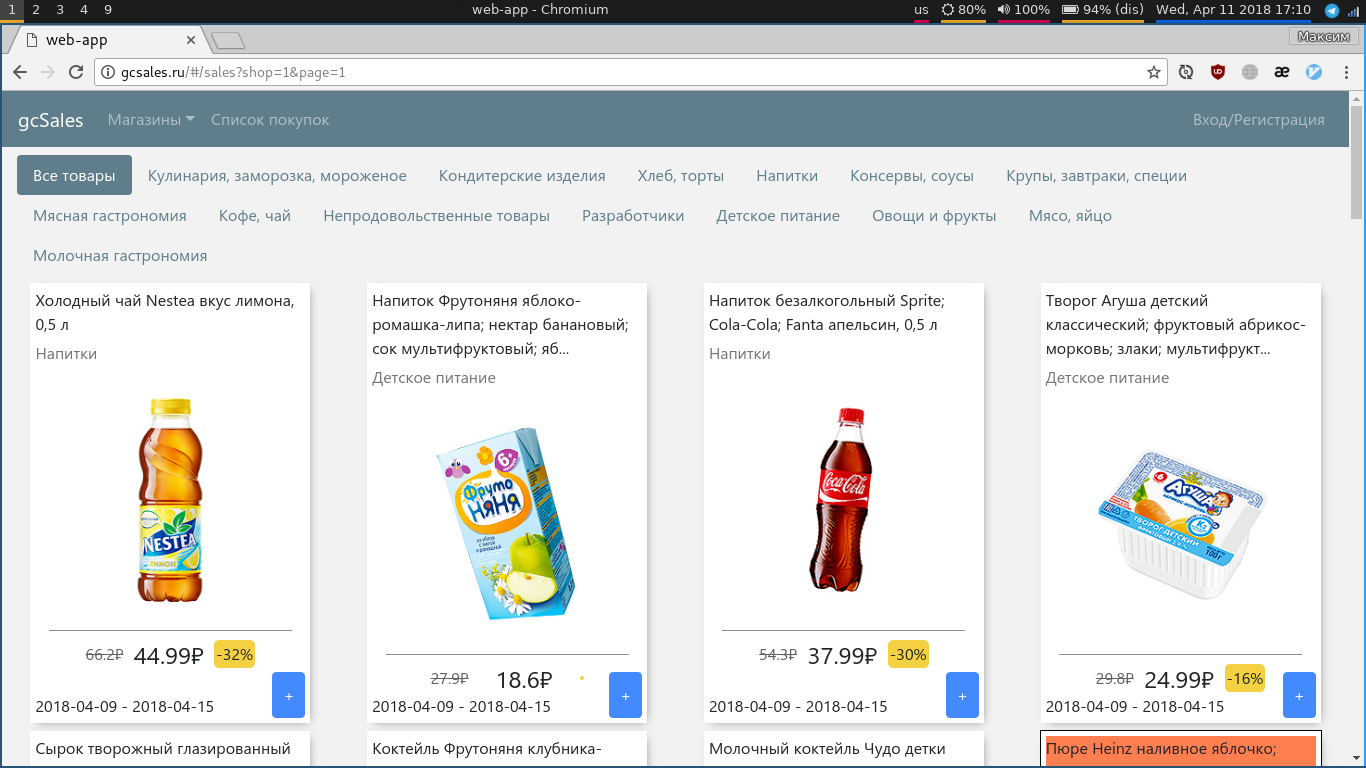
\includegraphics[width=\textwidth]{./screenshots/interface_main.png}
    \caption{Интерфейс полной версии }
    \endminipage
    \vspace{2cm}
    \minipage{0.2\textwidth}
    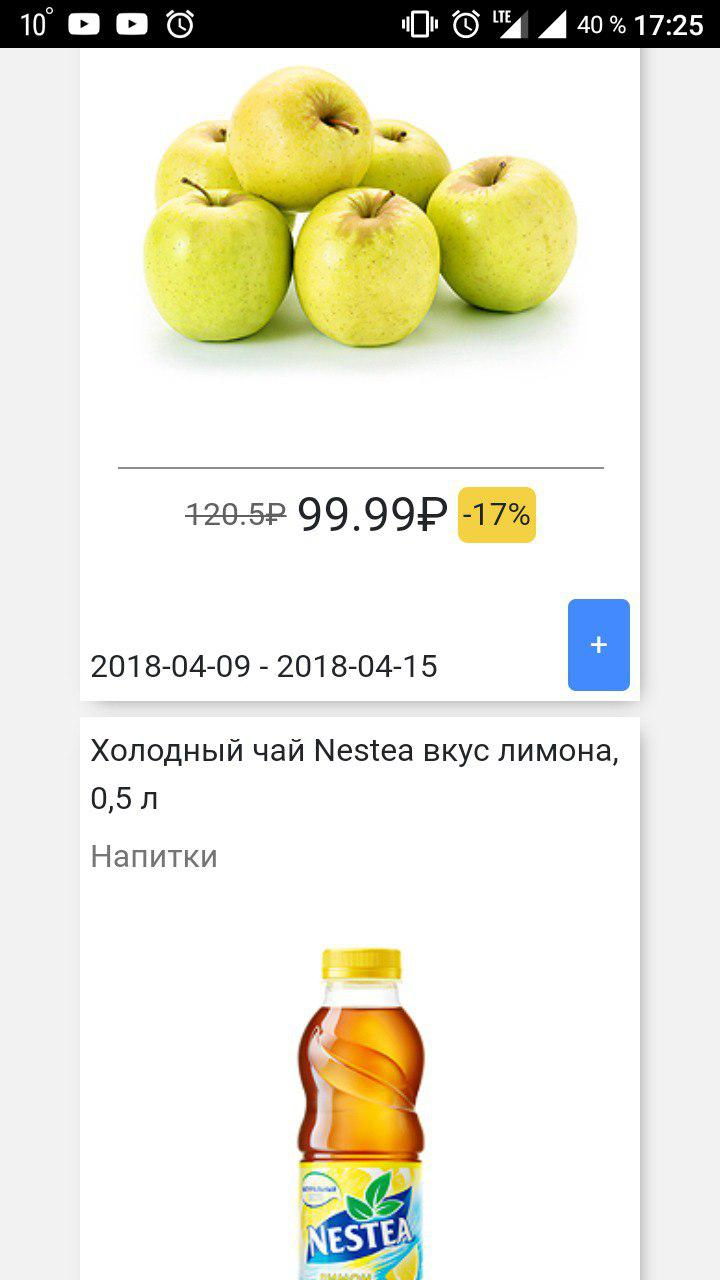
\includegraphics[width=\textwidth]{./screenshots/interface_small.jpg}
    \caption{Интерфейс мобильной версии}
    \endminipage
\end{figure}

% \begin{figure}[H]
%     \centering
%     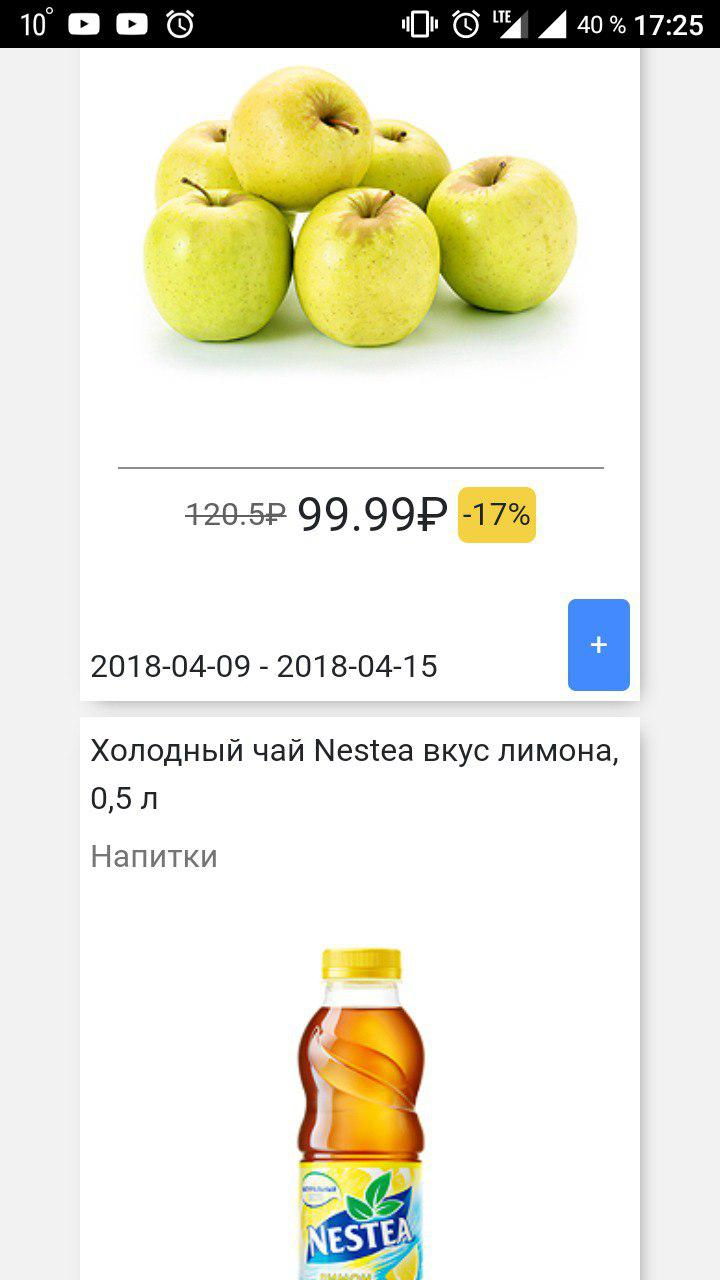
\includegraphics[width=0.3\textwidth]{./screenshots/interface_small.jpg}
%     \caption{Интерфейс мобильной версии}
% \end{figure}

\newpage
\subsection{Проверка требований к функциональным характеристикам}
\subsubsection{Веб-приложение}

По умолчанию должны отображаться товары всех категорий (см. Рис. 3), а при
нажитии на кнопку соответствующей категории должны отображаться только товары
этой категории (см. Рис. 4).

\begin{figure}[H]
    \centering
    \minipage{0.49\textwidth}
    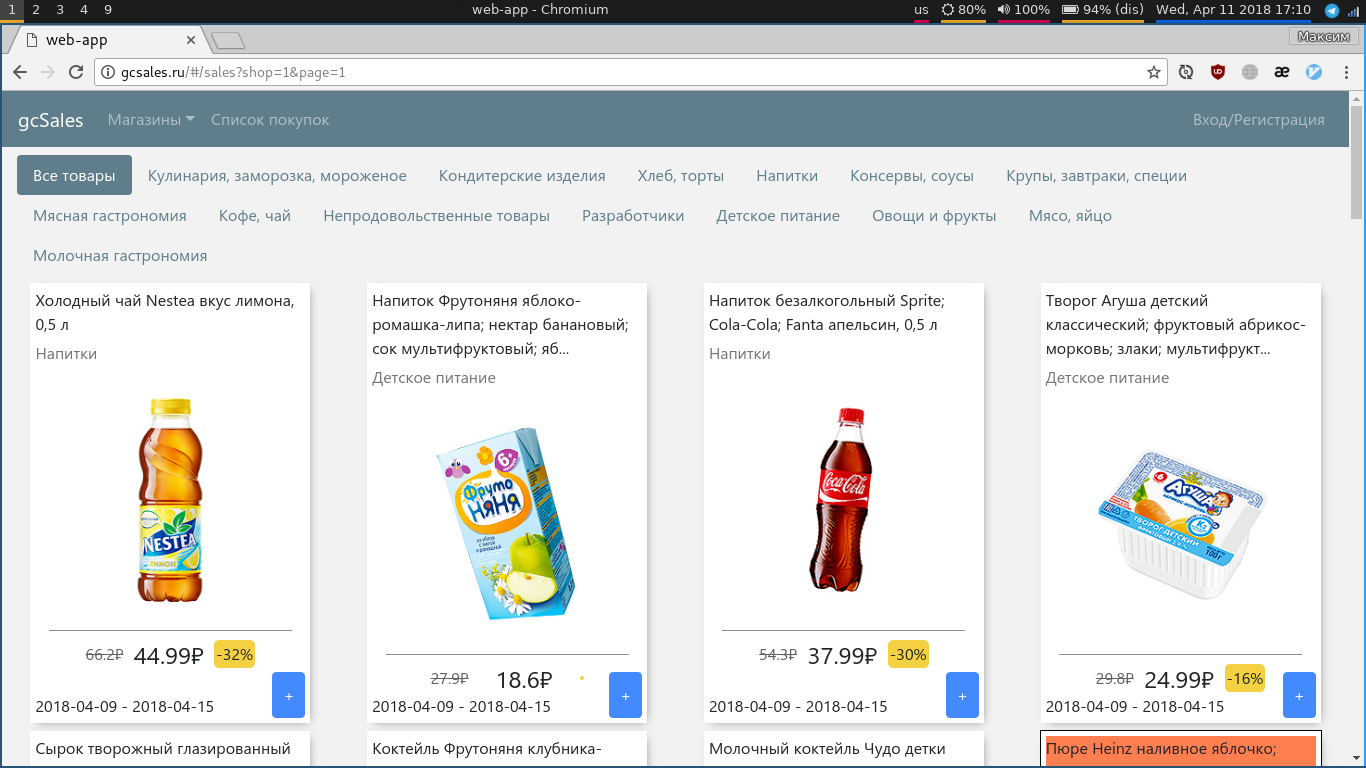
\includegraphics[width=\textwidth]{./screenshots/interface_main.png}
    \caption{Просмотр товаров в виде общего списка}
    \endminipage\hfill
    \minipage{0.49\textwidth}
    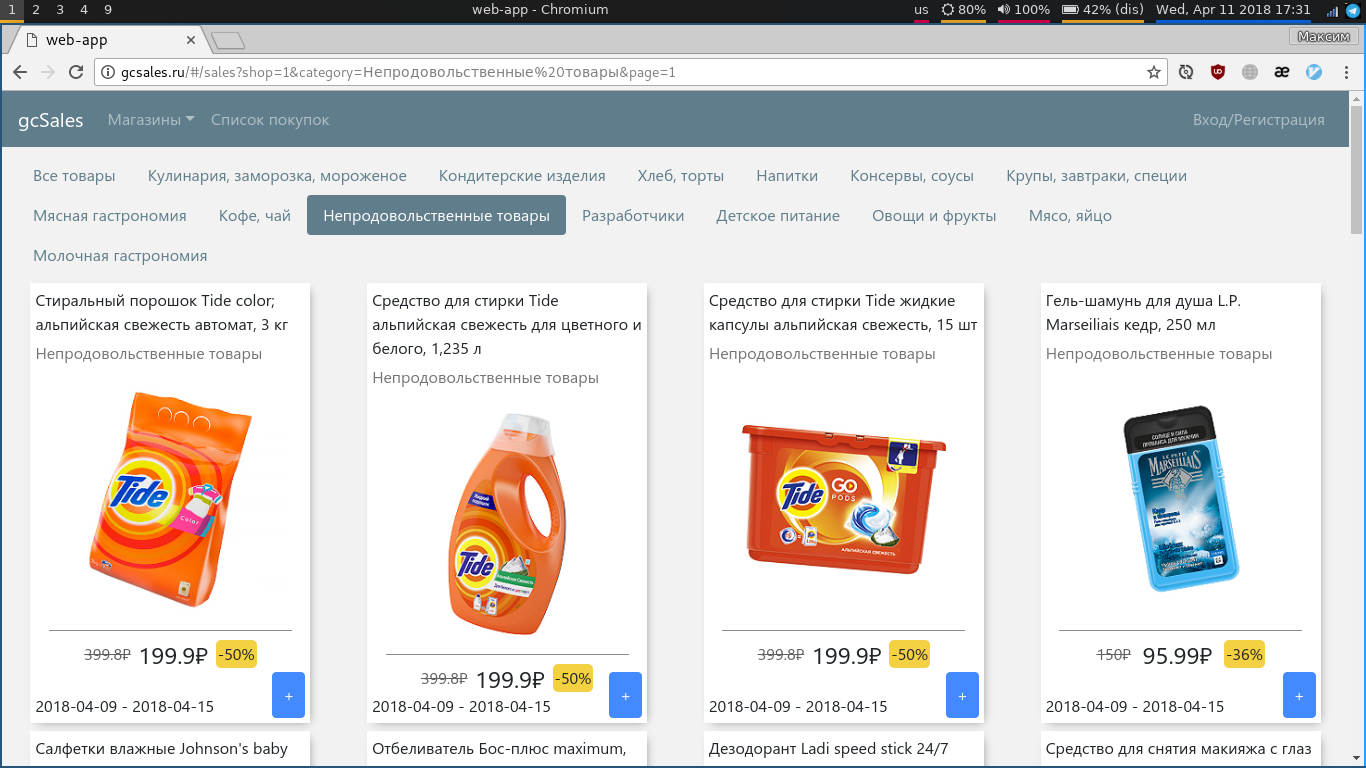
\includegraphics[width=\textwidth]{./screenshots/categories.png}
    \caption{Просмотр товаров категории "Непродовольственные товары"}
    \endminipage
\end{figure}

При нажатии на кнопку "Вход/Регистрация" должна отобразиться форма как на Рис.
5. Далее, если пользователь нажмет кнопку "Регистрация", то должна отобразиться
форма как на Рис. 6. Если пользователь введет верные данные, то система должна
переадресовать его на главную страницу, а кнопка "Вход/Регистрация" должна
изменить свой текст на "Выйти". После чего ему станет доступен список покупок.

\begin{figure}[H]
    \centering
    \minipage{0.49\textwidth}
    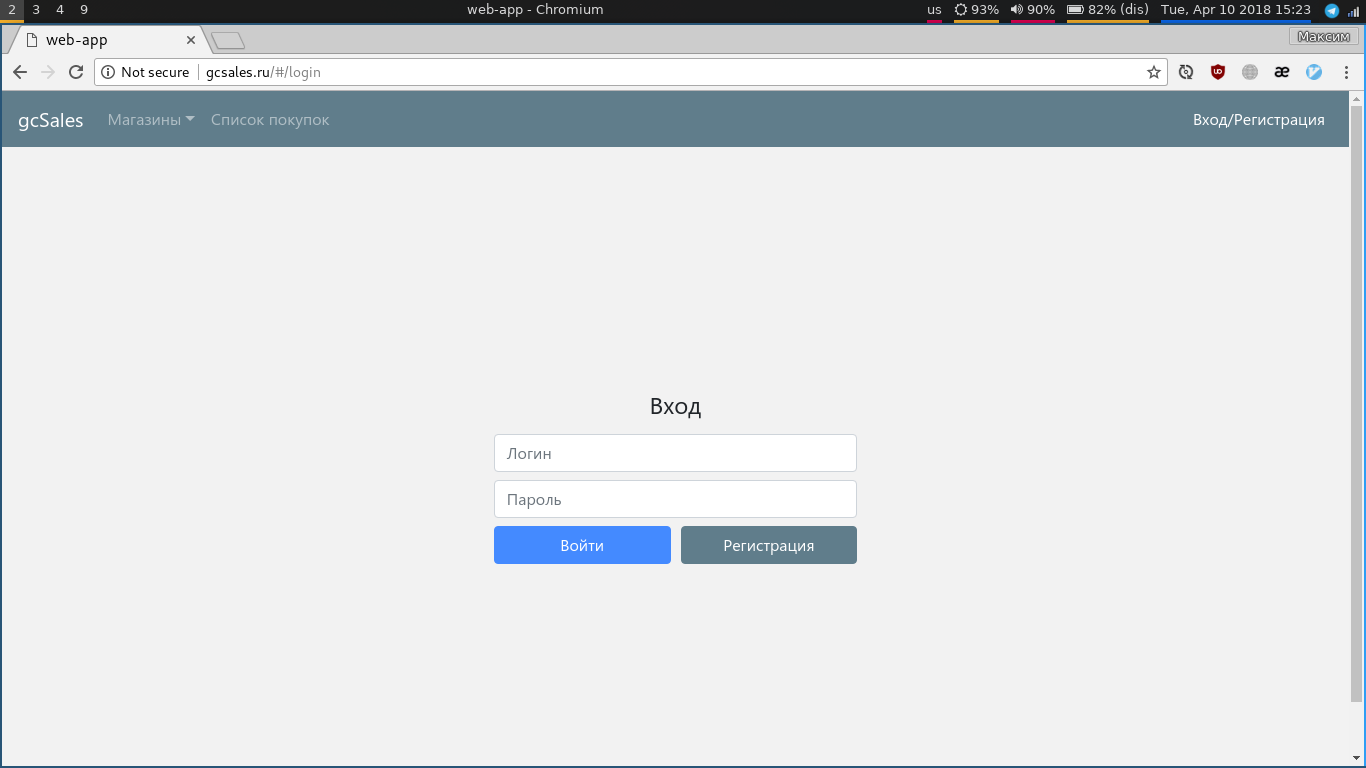
\includegraphics[width=\textwidth]{./screenshots/login.png}
    \caption{Авторизация}
    \endminipage\hfill
    \minipage{0.49\textwidth}
    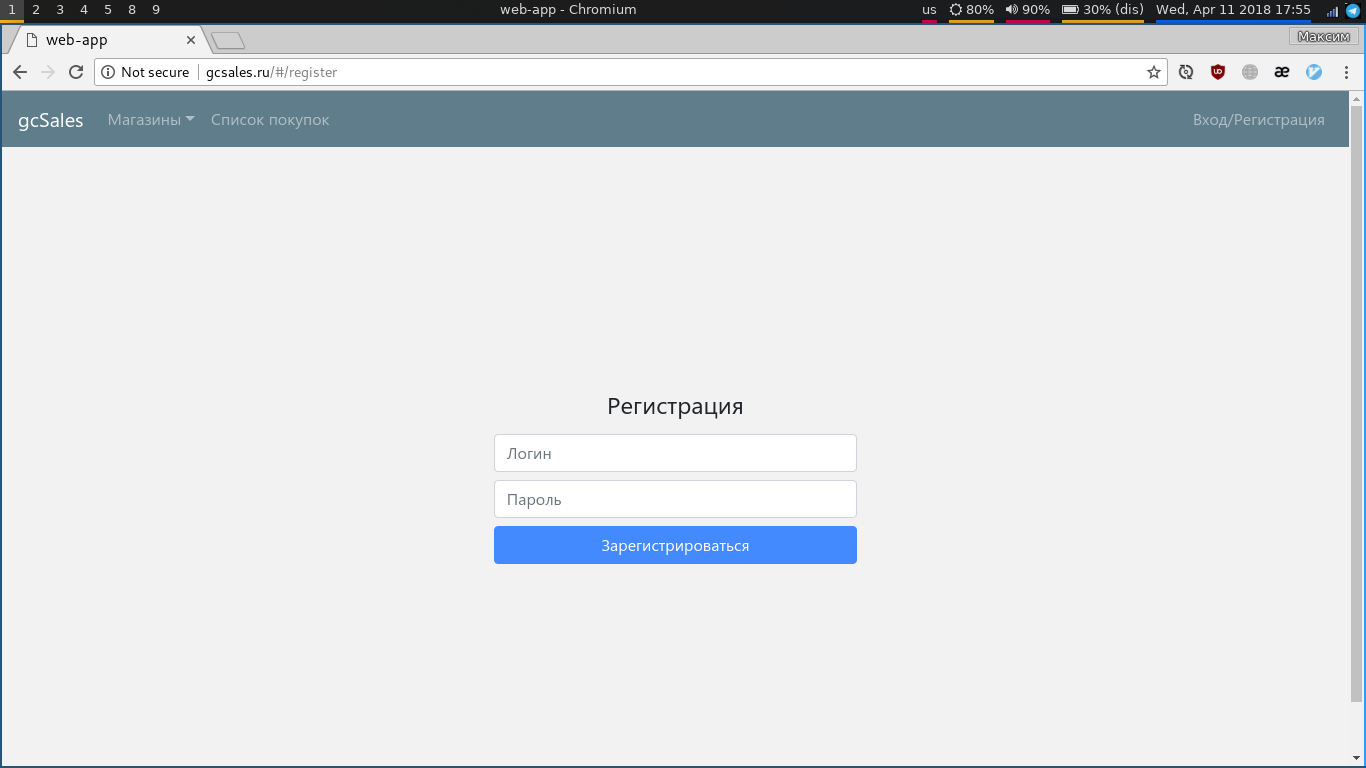
\includegraphics[width=\textwidth]{./screenshots/register.png}
    \caption{Регистрация}
    \endminipage
\end{figure}

В разделе "Список покупок" при нажатии на кнопку "Добавить" должен появиться
диалог как на Рис. 7. После ввода имени списка и нажатии "Ok" список покупок
должен появиться (Рис. 8).

\begin{figure}[H]
    \centering
    \minipage{0.49\textwidth}
    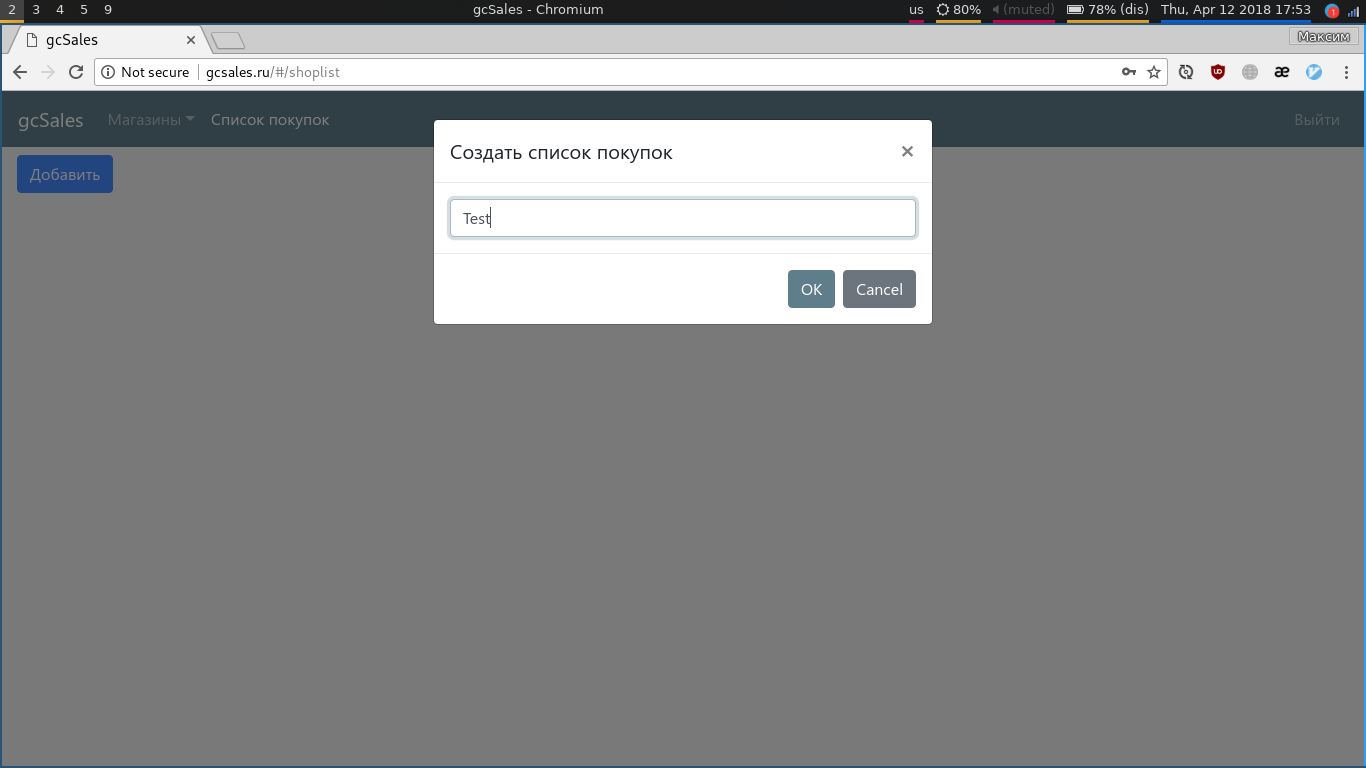
\includegraphics[width=\textwidth]{./screenshots/create_shoplist.png}
    \caption{Создание списка покупок}
    \endminipage\hfill
    \minipage{0.49\textwidth}
    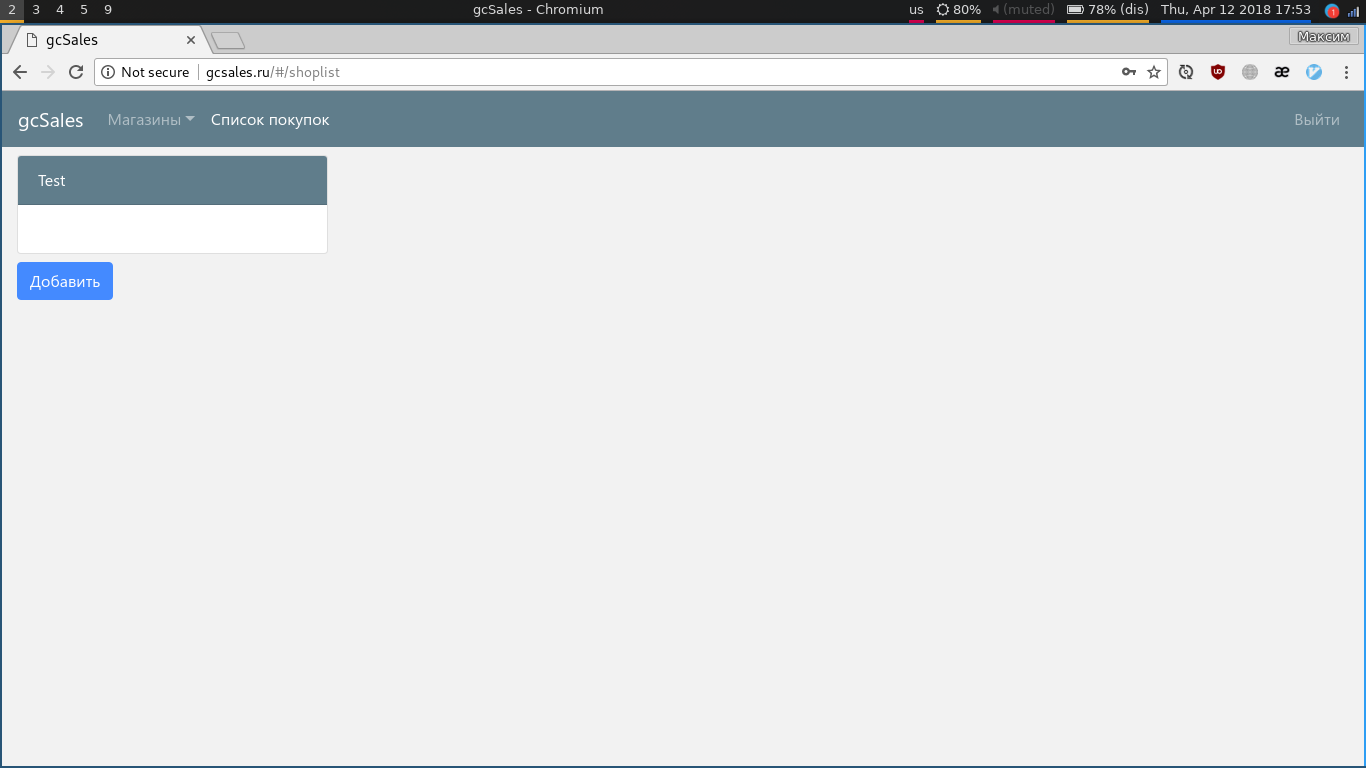
\includegraphics[width=\textwidth]{./screenshots/new_shoplist.png}
    \caption{Список покупок создан}
    \endminipage
\end{figure}

При нажатии на кнопку "+" в карточке товара должнен отобразиться диалог (Рис.
9). После выбора списка покупок, товар должен появиться в нем (Рис. 10).

\begin{figure}[H]
    \centering
    \minipage{0.49\textwidth}
    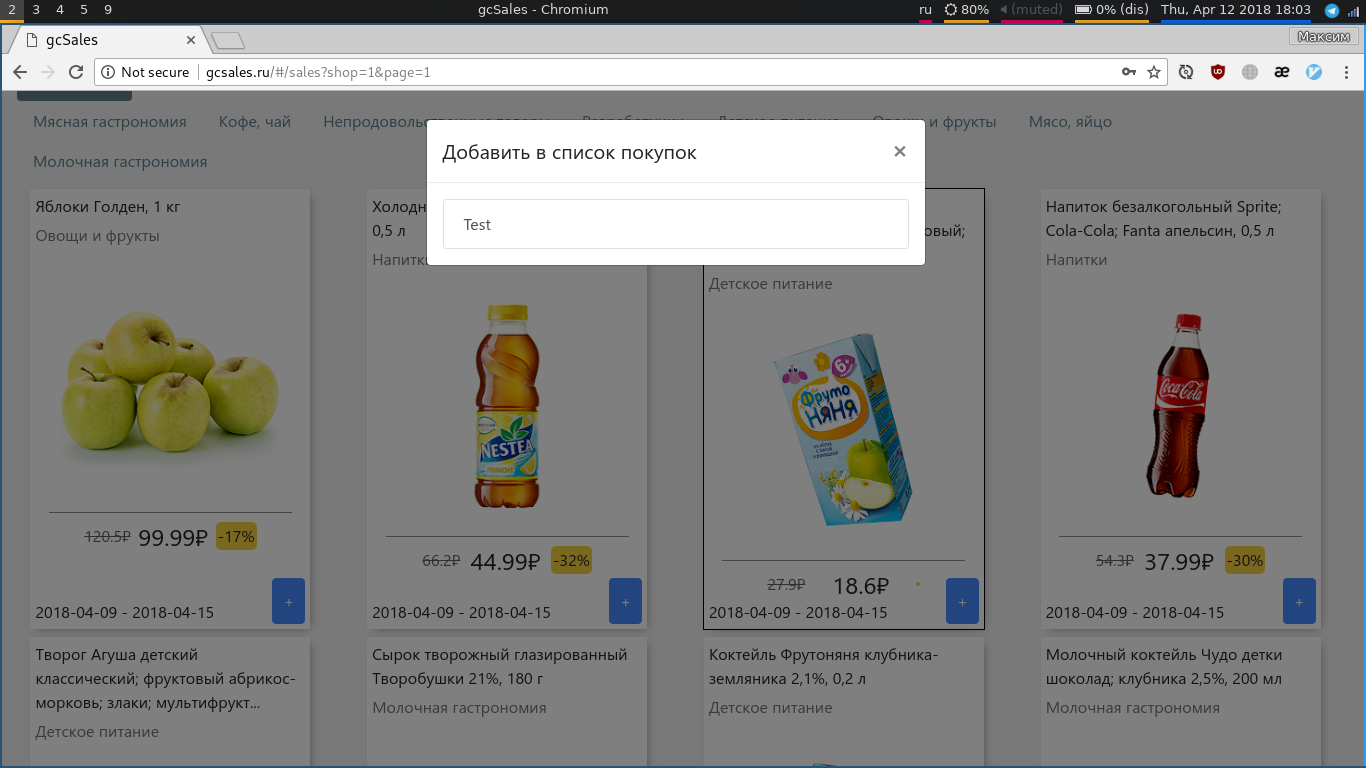
\includegraphics[width=\textwidth]{./screenshots/choose_shoplist.png}
    \caption{Выбор списка покупок}
    \endminipage
    \minipage{0.49\textwidth}
    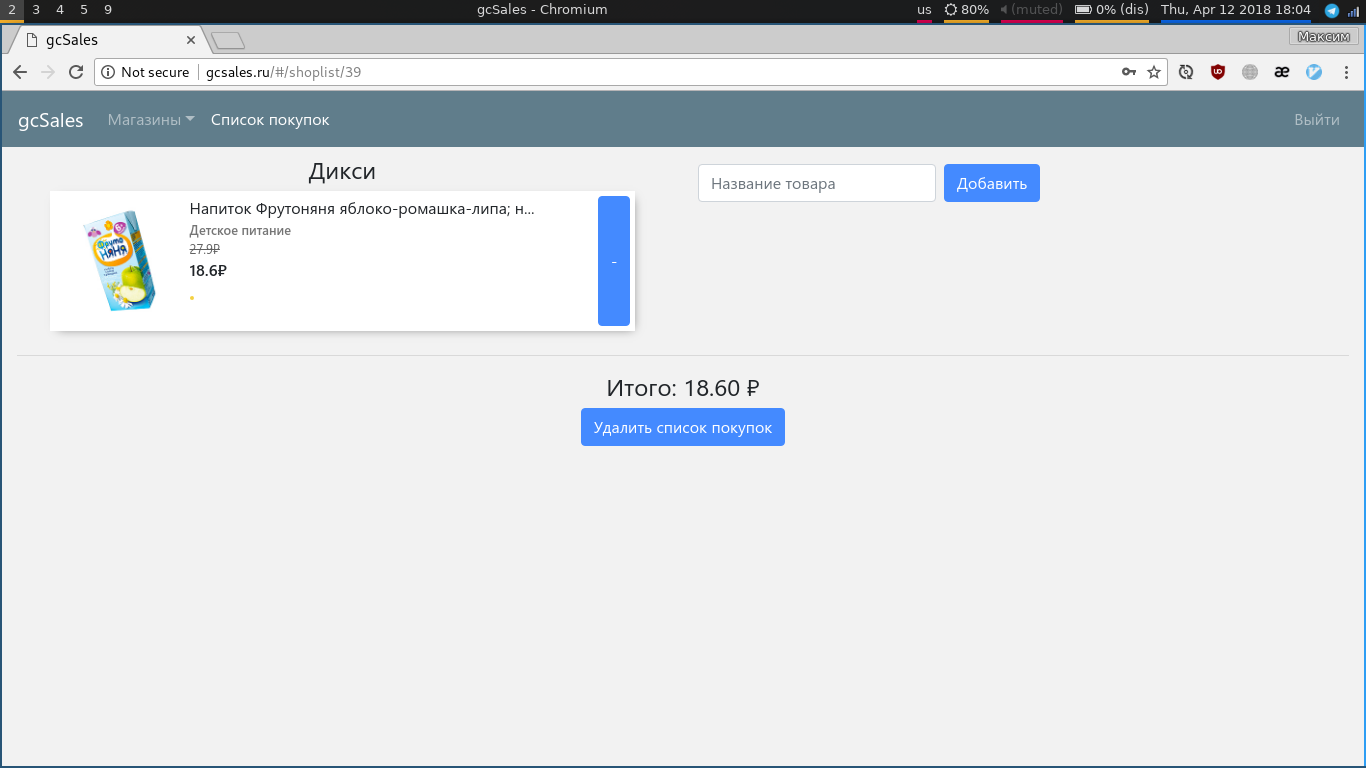
\includegraphics[width=\textwidth]{./screenshots/item_added.png}
    \caption{Товар добавлен в список покупок}
    \endminipage
\end{figure}

При вводе в поле пользовательской позиции (Рис. 11) и нажатии кнопки "Добавить"
она должна появиться в списке покупок, а также должны отобразиться рекомендации
для нее (если таковые нашлись). (Рис. 12)

\begin{figure}[H]
    \centering
    \minipage{0.49\textwidth}
    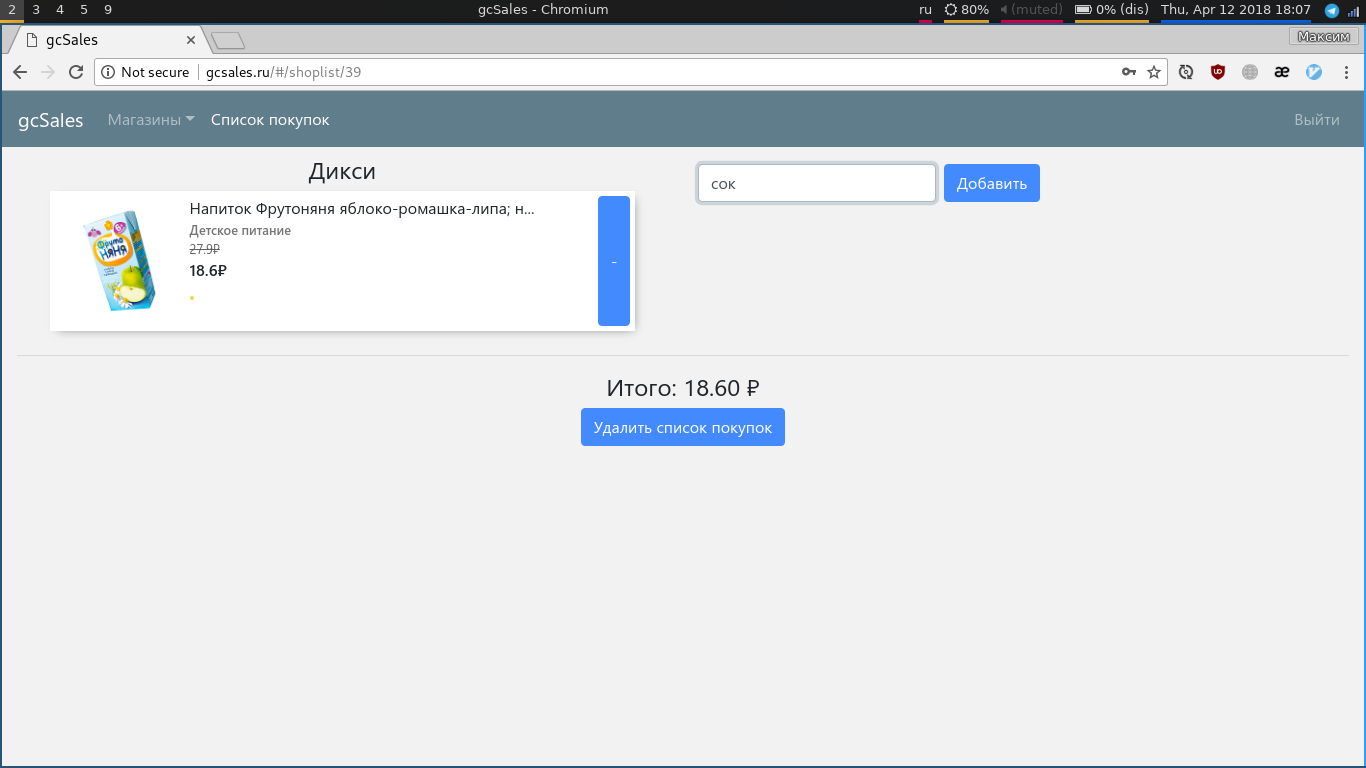
\includegraphics[width=\textwidth]{./screenshots/add_custom.png}
    \caption{Добавление пользовательской позиции}
    \endminipage
    \minipage{0.49\textwidth}
    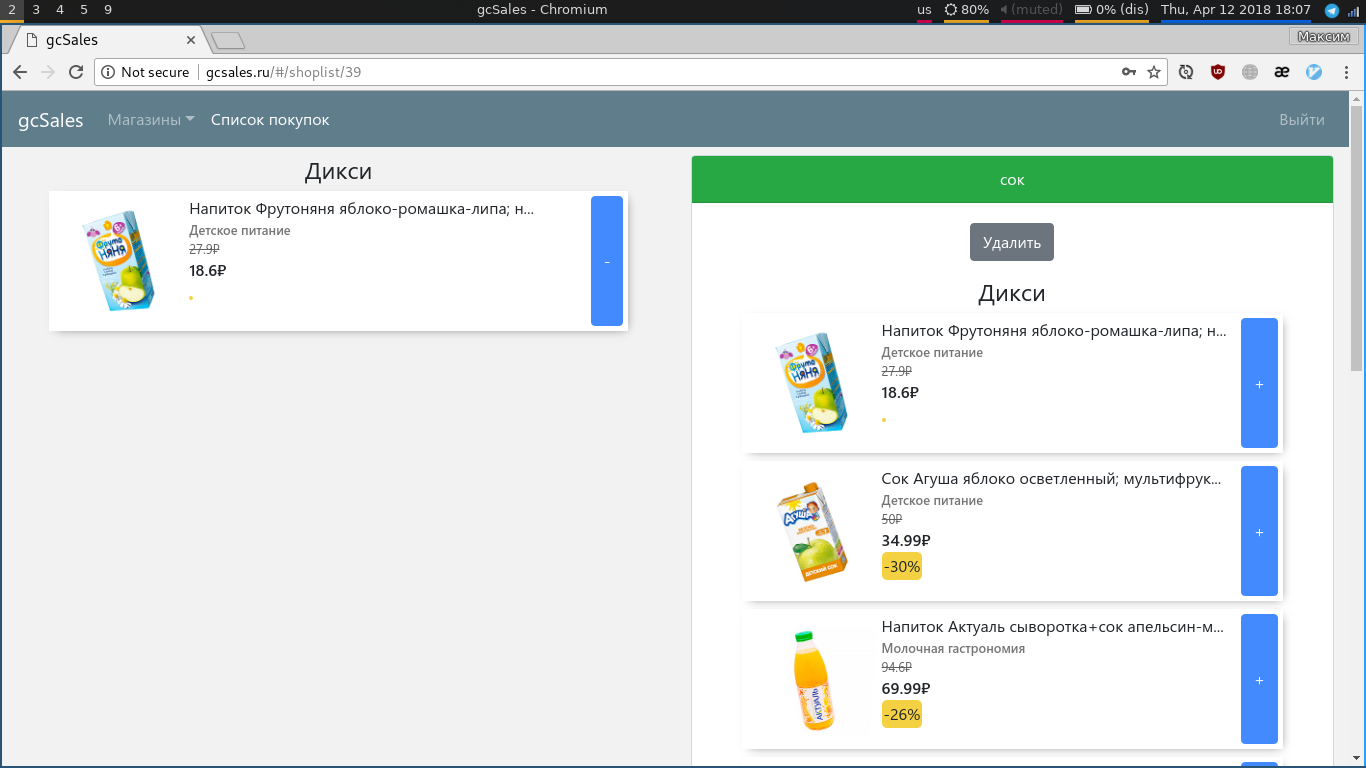
\includegraphics[width=\textwidth]{./screenshots/custom_created.png}
    \caption{Пользовательская позиция с рекомендациями}
    \endminipage
\end{figure}

При нажатии кнопки "-" на товаре из магазина, он должен удалится из списка
покупок. При нажтии кнопки "Удалить" пользовательская позиция должна удалиться.

\subsubsection{Серверное приложение}
При отправке любого запроса, описанного в Пояснительной записке, должен
возвращаться статус 200 в случае успеха и иной статус в случае неудачи.\\
Пример запроса:
\begin{figure}[H]
    \centering
    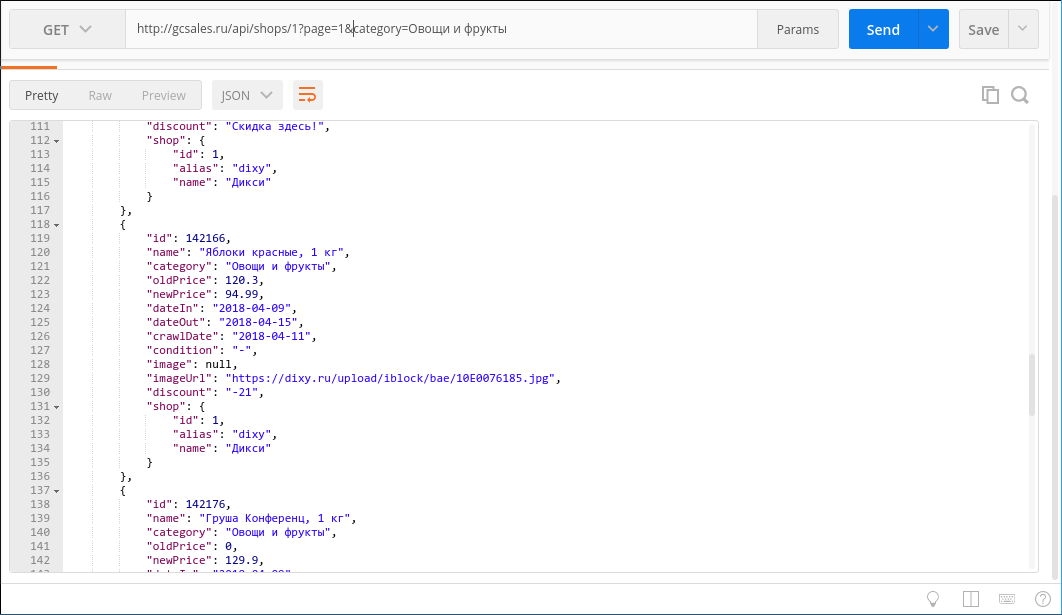
\includegraphics[width=0.7\textwidth]{./screenshots/postman.png}
    \caption{Отправка GET-запроса на сервер и получение ответа}
\end{figure}

\subsection{Проверка требований к временным характеристикам}
Для проверки требованиям к временным характеристикам должно быть проведено
несколько запросов для получения списка акций. Результат должен получиться
около того, что на Рис. 15 и не должен выходить за допустимые пределы,
описанные в Техническом задании.
\begin{figure}[H]
    \centering
    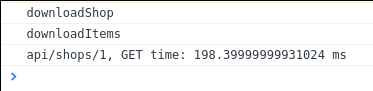
\includegraphics[width=0.5\textwidth]{./screenshots/get1.png}
    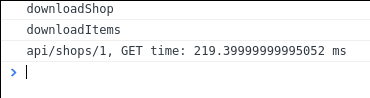
\includegraphics[width=0.5\textwidth]{./screenshots/get2.png}
    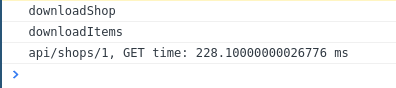
\includegraphics[width=0.5\textwidth]{./screenshots/get3.png}
    \caption{Замер времени отправки запроса}
\end{figure}

